\newcommand{\code}[1]{\texttt{#1}}

\chapter{Implementieren des hexagonalen Schachs nach Glinski}
Für die Implementierung des hexagonalen Schachs wird die Bibliothek \textit{pygame} genutzt. Diese vereinfacht es Spiele zu programmieren. Die Bibliothek stellt Methoden zur Verfügung, welche Fenster erstellen und Objekte malen. So eine Bibliothek erleichtert die Arbeit und ermöglicht einen schnelleren Start mit dem eigentlichen Programm. \textit{pygame} wird als Grundbaustein der Spieleprogrammierung in Python genutzt.

\begin{figure}[H]
    \centering
    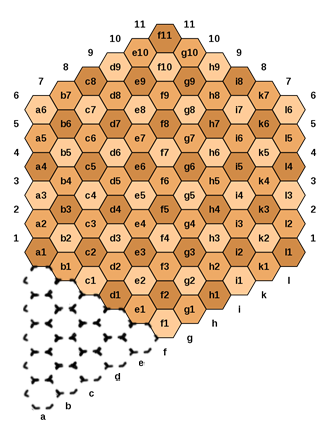
\includegraphics{images/hexIndex.png}
    \caption{Beschriftetes Spielfeld \protect\footnotemark}
    \label{fig:hex:index}
\end{figure}
\footnotetext{\url{https://commons.wikimedia.org/wiki/Category:Glinski\%27s_hexagonal_chess}}

Das Feld besteht aus 91 Hexagonen. Die Hexagone werden in einer zweidimensionalen Liste gespeichert. Mit dem ersten Index wird auf die Reihe, mit dem zweiten Index wird auf die Spalte zugegriffen. Mit den Indizes [0][0] wird das Feld  a6 angesprochen. Das nächste Feld in der Reihe ist bei b7 und wird mit den Indizes [0][1] angesprochen. Die Spalte a wird ab dem siebten bis zum elften Feld mit \textit{None} gefüllt, damit die Formatierung der Felder bleibt.\par
Das Feld ist eine eigene Klasse. Die Klasse hat die Attribute Stein und Nachbarn. Die Nachbarn sind oben-links, oben, oben-rechts, unten-rechts, unten und unten-links vom Feld. Die Attribute sind Referenzen zu den Feldern. Dazu werden die Felder auch noch in einer Liste gespeichert, welche per Index sich genau in der genannten Reinfolge aufrufen lassen. Die Nachbarn werden später für das Bewegen der Steine genutzt.\par
Ein Feld wird mit einer selbstgeschriebenen Methode markiert. Das Feld wird markiert, wenn ein Feld als Bewegungsmöglichkeit gilt. Ein Feld gilt als mögliches Feld, wenn die Figur nach den Regeln von Glinski sich auf das Feld bewegen kann. Die Methode zum Markieren eines Feldes sieht wie folgt aus.

\begin{lstlisting}[language=python,caption={Felder markieren},captionpos=b,label={lst:hexa:markieren},numbers=left,frame=none,escapechar=|]
def mark_tile(self, tile):
  if not isinstance(tile, GameBoard.Hexagon):|\label{m:line2}|
    return None

  if tile.piece is not None:
    if tile.piece.white is self.white:
      return "taken"

    GameBoard.Hexagon(tile.screen, tile.outer_radius, tile.inner_radius,tile.x_pos, tile.y_pos, (255, 0, 0))|\label{m:line9}|
    tile.piece.move_towards(tile.x_pos, tile.y_pos, False, False)
    tile.is_destination = True
    return "enemy"
  
  GameBoard.Hexagon(tile.screen, tile.outer_radius, tile.inner_radius, tile.x_pos, tile.y_pos, (249, 215, 28))
  tile.is_destination = True
  return "field can be destination"
\end{lstlisting}

Die Methoden nimmt als Parameter ein Feld an. Wenn der Parameter kein Hexagon ist, was in Zeile \ref{m:line2} abgefragt wird, wird \textit{None} zurückgegeben. Mit \code{if tile.piece is not None:} wird überprüft ob auf dem Feld ein Stein steht. In der If-Abfrage wird weiter abgefragt, ob der Stein die gleiche Farbe hat wie die Figur, mit welcher gespielt wird. Ist das der Fall, wird „taken“ zurückgegeben. Ist auch das nicht der Fall, geht das Programm weiter und kommt zu dem Teil wo das Feld markiert wird. Zeile \ref{m:line9} erstellt ein Hexagon auf der Position, wo das valide Feld liegt. Es muss ein neues Hexagon gemalt werden, da von dem alten nicht die Farbe geändert werden kann. Die Figur, die auf dem Feld stand, wird in diesem Prozess ebenfalls übermalt. Deswegen muss diese wieder in den Vordergrund bewegt werden. Das wird mit \code{tile.piece.move\_towards(tile.x\_pos, tile.y\_pos, False)} gemacht. Als letztes wird die Variable \textit{is\_destination} auf \textit{True} gesetzt. Diese Variable wird beim Klicken auf ein Feld abgefragt. Ist \textit{is\_destination True} wird der Stein auf das Feld bewegt, ist \textit{is\_destination False} passiert nichts. Am Ende des Rumpfes der If-Abfrage wird „enemy“ zurückgegeben. Nach der If-Abfrage folgen die Befehle, welche ausgeführt werden, wenn kein Stein auf dem Feld ist. Mit dem gleichen Befehl wird ein neues Hexagon gemalt. Dieses Mal ist die Farbe Gelb, anstelle eines Rots. Dadurch werden Felder mit Gegnern und freie Felder unterschieden. Ebenfalls wird die Variable \textit{is\_destination} auf \textit{True} gesetzt. Der Rückgabewert ist „field can be destination“.

\begin{lstlisting}[language=python,caption={Felder markieren},captionpos=b,label={lst:hexa:markieren},numbers=left,frame=none,escapechar=|]
def tile_remove_mark(self, tile):
  if not isinstance(tile, GameBoard.Hexagon):
    return None

  GameBoard.Hexagon(tile.screen, tile.outer_radius, tile.inner_radius,tile.x_pos, tile.y_pos)|\label{r:line5}|
  if tile.piece is not None:
    tile.piece.move_towards(tile.x_pos, tile.y_pos, True, False)

  tile.is_destination = False
  return "field no more destination"

\end{lstlisting}

\textit{tile\_remove\_mark} entfernt die Markierung wieder. Damit keine Fehler auftreten wird erst geprüft, ob der Parameter \textit{tile} wirklich ein Hexagon ist. Danach malt Zeile \ref{r:line5} das Hexagon mit der Standartfarbe. Wenn auf dem Feld eine Figur war, wird diese wieder nach vorne bewegt. \textit{is\_destination} wird wieder auf den Standartwert gesetzt.
